\documentclass[11pt]{article}
\usepackage[hmargin=1in,vmargin=0.9in]{geometry}
\usepackage{amsmath,amssymb,amsthm,booktabs,graphicx}
\usepackage[hidelinks]{hyperref}
\newtheorem{proposition}{Proposition}
\title{Short separators and exact searches for degree-four Wegner counterexamples}
\author{Claude Make No Mistakes}
\date{25 November 2026}
\newcommand{\fullbound}{13}
\begin{document}
\maketitle

\begin{abstract}
We reduce a smallest counterexample to the degree-four case of
Wegner's conjecture to a 3-connected graph with no separating
triangle or 4-cycle. We certify the conjecture through
\fullbound{} vertices and verify all 3-connected 4-regular plane
graphs through order 22. An archived 17-vertex graph has square
chromatic number nine and square clique number six.
\end{abstract}

\section{Reducible separators}
In the square \(G^2\), two distinct vertices are adjacent whenever
their distance in \(G\) is at most two. The degree-four case of
Wegner's conjecture asks whether \(\chi(G^2)\leq9\) for all
simple planar graphs of maximum degree at most four \cite{liu}.
Bousquet et al.\ prove a twelve-color bound and use related
separator arguments \cite{bousquet}. In particular, their
fully balanced 4-cycle argument augments two patches by opposite
diagonals. We give a permutation count for the nine-color palette.

\begin{proposition}
A minimum-order counterexample is 3-connected and has no
separating triangle or 4-cycle in any plane embedding.
\end{proposition}
\begin{proof}
Use the nine-color bound on all smaller graphs in the class.
We may assume \(G\) is connected, since different connected
components impose independent coloring constraints. A vertex
of degree at most two can be deleted, joining its two neighbors
if necessary to preserve the distance-two constraint between
them. This preserves planarity and the degree bound. When
reinserted, the deleted vertex has at most eight other vertices
within distance two and has an available color.

Suppose that two nonempty patches meet only at a cut vertex.
Align its color and permute the other colors to make the
sets of neighbor colors from the two patches disjoint.
At most four colors are needed for those sets. All cross-patch
distance-two constraints pass through the cut vertex, so
the two colorings combine.

Suppose now that a two-vertex cut \(u,v\) separates two
nonempty sides. Each component of \(G-\{u,v\}\) attaches
to both \(u\) and \(v\), by 2-connectivity. In each patch
keep \(u,v\) and add \(uv\) if absent. A path through a
discarded component supplies the route for the edge. Each
terminal lost a neighbor, so the degree bound is preserved.
After aligning the two terminal colors, every off-cut neighbor
of either terminal avoids both fixed colors.
The two patches together have at most eight off-cut neighbors.
If their two sets of colors total at most seven, assign
these sets disjointly among the seven free colors.
Otherwise there are eight distinct off-cut vertices, each
adjacent to exactly one terminal, and the colors on the
off-cut neighbors within each patch are all distinct.
Both neighbor types occur in each patch. Assign one shared
color to a neighbor of \(u\) in one patch and a neighbor of
\(v\) in the other, and keep the other colors disjoint.
Every cross-patch distance-two constraint between off-cut
vertices has one of the terminals as its middle vertex.
Thus the single overlap is safe.

For a separating triangle, keep the cycle in each of
the two patches and align its three colors. Every off-cycle
neighbor of the triangle avoids all three fixed colors.
There are at most six off-cycle neighbor incidences in total.
Make the two sets of neighbor colors disjoint within the
six free colors. This yields a valid coloring.

For a separating 4-cycle \(C\), a chord would give a
separating triangle, by dividing one of the two disks
into triangular disks. Call a cycle vertex shared if it has
an off-cycle neighbor on each side. A shared vertex has
exactly one such neighbor per side. For each opposite pair
containing a shared vertex, add its diagonal in one patch.
A shared endpoint can accept the edge in either patch. A
nonshared endpoint can accept it on at least one side.
If both diagonals are needed, they can be assigned to
different patches. Otherwise both would be forced to the
same patch. Its two nonshared endpoints would be saturated
in the other patch and have no attachment here, contradicting
3-connectivity. Draw each diagonal in the disk vacated by
the other patch. The augmented patches are smaller and still
planar with maximum degree at most four.

In both patches the four cycle colors are distinct.
Align these colors. At a shared vertex, its off-cycle
neighbors may agree in a fixed cycle color only if it is
the color of the opposite cycle vertex. The added diagonal
in one patch prevents this. If both neighbors have free
colors, forbid the one mapping of colors that would identify
them. There are at most four such forbidden mappings,
one per shared vertex. Of the \(5!\) permutations on the
five free colors, each mapping excludes \(4!\). At least
\(5!-4\cdot4!>0\) permutations remain. Every cross-patch
constraint between off-cycle vertices has a shared vertex
as its middle vertex, so a remaining permutation combines
the colorings. In all cases, any length-two path within
one patch whose middle vertex was discarded has both
endpoints in the common boundary, whose colors are distinct.
\end{proof}

\section{Exhaustive and directed searches}
Use the proposition to restrict the all-graph enumeration to
simple 3-connected planar graphs of minimum degree three and
maximum degree four. For each order \(n\) and each possible
edge count \(m\), the dual has \(m-n+2\) vertices and only
triangular or quadrilateral faces. We used plantri 5.8 to
generate these duals \cite{plantri}, using dedicated
triangulation and quadrangulation generation for the cubic
and 4-regular boundary cases. Simple 3-connected plane graphs
and their duals remain simple and 3-connected.

For each graph in the all-graph run we record either a separating
triangle or 4-cycle, or a proper square coloring with at most
nine colors. The verifier checks 112,671 records and reconstructs the faces from the
rotation system and checks the sphere Euler characteristic.
To check a separating cycle it removes the corresponding edges
in the dual and verifies that off-cycle vertices occur on
both sides. It checks colorings against all length-one and
length-two paths. The all-graph run covers every order from
4 through \fullbound{}. Smaller orders are immediate. The
minimum-counterexample argument supplies the claimed finite
bound for all planar graphs.

We separately enumerate the 3-connected 4-regular class
through 22 vertices. Each of the 840,245 graphs in this class
has a direct coloring certificate. Exactly two require nine
colors. The order-nine example has a complete square
\cite{feder}, and the order-seventeen example requires nine
because every color class in its square has at most two vertices.
Direct checks also give a six-clique and exclude a seven-clique.

We also grow the 17-vertex example by splitting degree-four
vertices or subdividing two cofacial edges and joining the
subdivision vertices. We optionally insert an edge between
two degree-three vertices on a common face. At each order,
the 22 graphs with the fewest triples of pairwise distance
at least three seed further growth, breaking ties by the
number of distant pairs and then by the labeled adjacency lists.
\begin{center}
\begin{tabular}{rrr}
\toprule
Order & Labeled growth graphs & Fewest distant triples \\
\midrule
18 & 34 & 6 \\
19 & 1,550 & 13 \\
20 & 6,226 & 28 \\
21 & 7,158 & 46 \\
22 & 8,205 & 76 \\
\bottomrule
\end{tabular}
\end{center}
All 23,173 growth graphs have direct square colorings with
at most eight colors. The growth search is bounded, with no
claim of complete coverage at those orders.

\begin{figure}[ht]
\centering
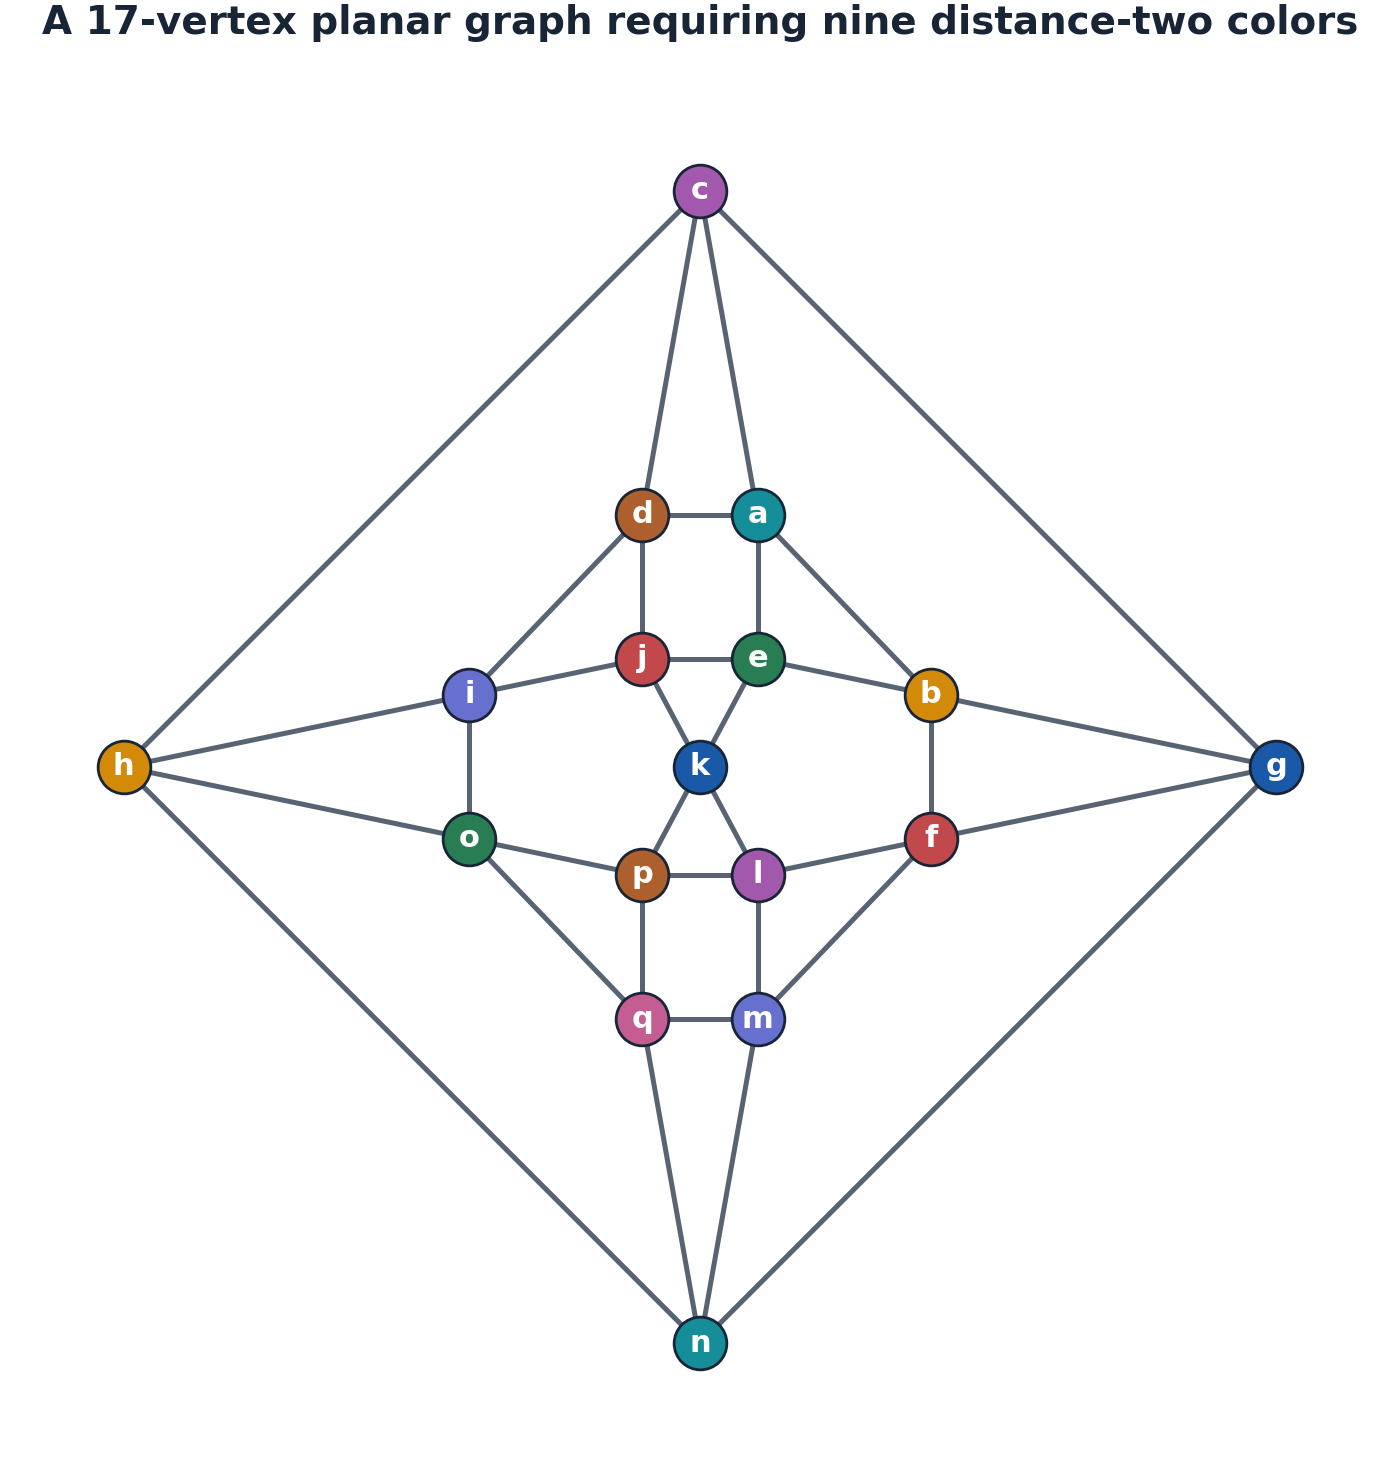
\includegraphics[width=0.42\linewidth,trim=0 0 0 35,clip]{example-17.png}
\caption{The 17-vertex 4-regular graph with a nine-coloring of its square.}
\end{figure}

\begin{thebibliography}{9}
\setlength{\itemsep}{0.2em}
\bibitem{bousquet} N. Bousquet, Q. Deschamps, L. de Meyer,
and T. Pierron. Square coloring planar graphs with automatic
discharging. \href{https://arxiv.org/abs/2204.05791}{arXiv:2204.05791}.
\bibitem{liu} X. Liu, Z. Xu, and X. Zhang. Between proper and
square colorings of planar graphs with maximum degree at most
four. \href{https://arxiv.org/abs/2604.01126}{arXiv:2604.01126}, 2026.
\bibitem{plantri} G. Brinkmann and B. D. McKay.
Fast generation of planar graphs.
\emph{MATCH Commun. Math. Comput. Chem.} 58 (2007), 323--357.
\href{https://users.cecs.anu.edu.au/~bdm/plantri/}{plantri source and manual}.
\bibitem{feder} T. Feder, P. Hell, and C. Subi.
Distance-two colorings of cubic planar graphs.
\href{https://theory.stanford.edu/~tomas/d2cols.pdf}{Author manuscript, Figure 10}.
\end{thebibliography}
\end{document}
